\chapter{Theoretical background}
%Some intro? recap motivation? PR 3 St 2
Our goal, is to add the final steps in the theory chain which transforms the GRMHD simulations into interferometric observables. For this to be achieved and for the theory higher up in the chain to be maximally useful in data interpretation, realistic signal corruptions need to be considered. Hence, the purpose of this module is to further the sophistication of the interplay between theory and observation in the field.\\
~\\
%The plan for the chapter? PR 3 St 2
The signal corruptions which we have identified as the most prominent occurs in the troposphere, interstellar medium (ISM) and within the stations themselves. First I will review some EM wave fundamental and introduce scattering theory, which is applicable to both the radiative process occuring in the troposphere and ISM. Following the general introduction I will explore each specific case.\\

\subsection{Radio Interferometry}
%Define basic radio interferometry concepts which are used later. (don't over do) PR 2 St 3

van-citterlike theorem a relationship between the image of the sky and it's fourier transform.

\begin{equation}\label{eq:vis_im}

van-citterlike theorem

\end{equation}•


Briefly introduce interferometry. Necessity of interferometry to obtain adequate
resolution.
Define Fourier transform relationship between image - visibilities.


\subsubsection{Measurement Equation}
%PR 2 St 3
Signal propagation and Jones matricies.

\subsubsection{mm-VLBI observables and data products}
%PR 2 St 2
Visibility amplitudes, closure quantities, polarisation ratios, and images.
If the visibility phase is highly variable as in the case of a turbulent atmosphere,  conventional calibration and imaging techniques have severely limited (if any) success. However information can still be extracted from the raw visibilities in the form of closure quantities \citep{Monnier_2007} or polarisation ratios \citep{Fish_2009}. Closure phase, defined as the sum of 3 visibility phases of a triangle of stations $\left\{i,j,k\right\}$, is a probe of asymmetry in source structure,
\begin{equation}
\Phi_{ijk} = \phi_{ij}+\phi_{jk}+\phi_{ki}.
\end{equation}

\noindent Because most signal corruptions are station based, the gain phase terms $\phi_{ij}=\phi^{\rm true}+ \phi^G_i -\phi^G_j$ for each antenna will cancel, yielding a more robust observable. 

The uncertainty on the closure phase is model dependent \citep{Rogers_1995} and is given as a function of the SNR $s$ of each baseline 

\begin{equation}\label{eq:ucp}
u(\Phi_{ijk}) = \frac{\sqrt{4 + (s_{ij}s_{jk})^2 + (s_{jk}s_{ki})^2 + (s_{ij}s_{ki})^2 +
                        2(s_{ij}^2+s_{jk}^2+s_{ki}^2)}}{s_{ij}s_{jk}s_{ki}},
\end{equation}

\noindent where $s_{ij}$ is defined as
\begin{equation}
s_{ij}=|V_{ij}| \sqrt{\frac{ \tau \Delta \nu}{SEFD_i SEFD_j}},
\end{equation}
where $\tau$ is the vector averaging timescale, $\Delta \nu$ is the bandwidth, $|V_{ij}|$ is the visibility amplitude and $SEFD$ is the system equivalent flux density. The result that closure phase is entirely immune to station based effects breaks down however when time averaging in the presence of baseline dependent effects like thermal noise as illustrated in section~\ref{closure_errors}.
 
 \subsubsection{Variability and the static source assumption}
%PR 1 St 2

%the assumption
Implicit in our description of interferometry above, we assumed that the source remains approximately unchanged or static during the course of the observation. However, if this assumption does not hold (i.e. if the source is time-variable),  the visibilities measured over the course of an observation can no longer be related to a single image and if they are, the resulting image would appear smeared out as it is averaged over many realisations. 
%explicitly defining variability
Note that I am using the term `variability' in a general sense which refers to changes in any source observables. Most commonly variability is refers to changes in source flux (visibility amplitude) but I include changes in source structure and position (visibility phase) and source polarisation. Practically it is difficult to separate source and instrumental variability without accurate models and measurements for all non-source signal propagation effects. Models of several signal corruptions will be discussed in later chapters but here it is relevant to repeat that time variability of each corruption is emphasised in our theory and simulation. In addition the simulator allows for the input source to be generically variable. 
%Observed variability from SgrA
Although the static source assumption holds for most interferometric observations, the accretion flow and magnetic field structures around a SMBH can be variable on far shorter timescales.  In particular, Sgr~$^\star$ exhibits variability on timescales of minutes to hours in the radio (including mm-VLBI), near-infrared, and X-ray bands (Doeleman 2009 and references therein, Fish_2009, Johnson_2015b). This wealth of observational data has yielded several answers but the origin of the variability is still highly debated. To explain the observed delay between flares in different bands an expanding plasma model (Marrone, 2008) is often used. One intriguing observational result is that variability in the polarisation domain is far more rapid than the total intensity. 

%Light crossing analysis
ISCO depends on spin so maybe can constrain spin through periodic orbital features
In principle, the variability timescale can be comparable to the period of the Innermost Stable Circular Orbit (ISCO), which for Sgr~A$^\star$, ranges from 4 minutes for a maximally rotating BH to about half an hour for a non-rotating BH. M87 ISCO is longer ~ dConsidering light crossing times $\Delta t_{\rm cross}$, we can estimate the angular size $\theta$ of the emission region to be of order $\theta \sim \Delta t_{\rm cross} c /D_{\rm src}$, where c is the speed of light and $D_{\rm src} is the observer-source distance. Hence for Sgr~$^\star$ at a distance of $8.3$~kpc (Gillessen, 2009), for a flare of duration $ \Delta t_{\rm cross} =10$~min, $\theta =  variability   which corresponds to scales of  $15 R_{\rm Sch}$  light-crossing times of . 

Early EHT observations of Sgr~A$^\star$ already showed significant inter-day variability in total intensity \cite{Fish_2009}. The variability timescale is much shorter in polarisation which detect intra-hour variability of fractional polarisation \cite{Johnson_2015b}.  and  Johnson (2014) shows that even with few baselines, the astrometry of a compact flaring component can be well constrained. 

%There are some ways to track/mitigate variability but this is beyond scope
Depending on the science goals, variability can either be a target or an obstacle to the observation. If a flare is dominated by a localised variable structure, several approaches \citep{Doeleman_2009, Johnson_2014} show that EHT can track flaring structures using closure quantities and polarimetric ratios which could help map the spacetime around the BH. Alternatively \citet{Lu_2016} show that a gaussian weighting scheme can  mitigate the effects of variability so that the shadow can still be measured although approach would downweight the longest baselines. An extensive discussion on analysis and interpretation of variability is out of the scope of this thesis.


conversation with Jeandrew - hotspot if in a resonant orbit, would not be sheared as the orbital frequency is constant within the resonance. easier example of orbital resonance is saturn's rings 

From Fish 2011:
``
Broad band flares:
(Marrone
et al. 2008; Yusef-Zadeh et al. 2009; Dodds-Eden et al. 2009)

For previous sub-mm observations which show variability of SgrA*: 
Marrone et al. 2006; Yusef-Zadeh et al. 2009;
Kunneriath et al. 2010

While a low expansion speed is predicted by
models of adiabatically expanding source components (Eckart
et al. 2008, 2009; Yusef-Zadeh et al. 2009), these models also
5The Astrophysical Journal Letters, 727:L36 (6pp), 2011 February 1
Fish et al.
predict an increase in source size. Our observations detect
Sgr A* after the increase in flux density has occurred, but we do
not find evidence of an increase in source size as predicted by
adiabatic expansion. Future, more sensitive observations of Sgr
A* before, during, and after a flare event will be necessary to
more fully understand the mechanism responsible for variability
in Sgr A*.
``

\subsection{Scattering basics}
%PR 1 St 2
% Similiar to paper Fig. An illustration of basic scattering in the strong and weak regimes PR 1

Millimetre wavelength radiation originating at the Galactic Centre is repeatedly scattered along the signal path to the Earth-based observer. The first occurrence is due to electron plasma in the interstellar medium (ISM) (\citealt{Bower_2006}, \citealt{Gwinn_2014}), while the second is due to poorly-mixed water vapour in the Earth's troposphere (\citealt*{Carilli_1999}, \citealt*{Lay_1997}). It is essential that the effects of the scattering phenomena are understood for a rigorous calibration and interpretation of data.  Towards this end, simulation modules approximating scattering in both media are implemented in \textsc{MeqSilhouette}. As an introduction to the separate descriptions of each, we review a simple scattering model.


An electro-magnetic wave is scattered when it passes through a medium with refractive index inhomogeneities. Following \citet{Narayan_1992}, this effect can be modeled as a thin screen, located between source and observer planes and orientated perpendicular to the line-of-sight. The screen, indexed by coordinate vector $\mathbf{x}$, adds a stochastic phase $\phi(\mathbf{x})$ to the incoming wave at each point on the screen, yielding a corrugated, outgoing wavefront. We define the Fresnel scale as  $r_{\rm F} = \sqrt{\lambda D_{\rm os}/2\pi}$, where $D_{\rm os}$ is the observer-scatterer distance, or the distance where the geometrical path difference $\frac{2\pi}{\lambda} (D_{\rm os} - \sqrt{D_{\rm os}^2 + r_{\rm F}^2}) =\frac{1}{2}$~rad.


To determine the resultant electric field at a point in the plane of the observer, indexed by coordinate vector $\mathbf{X}$, one has to take into account all possible ray paths from the screen to $\mathbf{X}$. To illustrate the model, a calculation of the electric field amplitude, $|E(\mathbf{X})|$ yields the Fresnel-Kirchoff integral \citep*{BORN_1980}
\begin{equation}\label{Fresnel- Kirchoff}
|E(\mathbf{X})| = C \int_{\rm screen} \exp\left[i\phi(\mathbf{x}) + i \frac{(\mathbf{x}-\mathbf{X})^2}{2 r_{\rm F}}\right]\mathbf{dx},
\end{equation}
where C is a numerical constant.


The statistics of $\phi(\mathbf{x})$ can be described by a power spectrum or equivalently the phase structure function,
\begin{equation}\label{eq:D_phi}
D_\phi (\mathbf{x},\mathbf{x'}) = < \left[ \phi(\mathbf{x} +\mathbf{x'}) - \phi(\mathbf{x})\right]^2 >,
\end{equation}
where $\mathbf{x}$ and $\mathbf{x'} $ represent two points on the screen and $<>$ denotes the ensemble average. 

There is evidence that $D_\phi$ can be reasonably approximated by a power law dependence on the absolute distance $r$ between points on the screen  \citep{Armstrong_1995,carilli_1997}
\begin{equation}
D_\phi (r) =  (r/r_0)^\beta,\qquad r^2 = \mathbf{x}^2 - \mathbf{x'}^2
\label{kolmogorov}
\end{equation}
where $r_{\rm 0}$ is the phase coherence length scale defined such that $D_\phi(r_{\rm 0}) = 1$~rad. 

Kolmogorov turbulence, which describes how kinetic energy injected at an outer length scale $r_{\rm out}$ cascades to increasingly smaller scales until finally dissipated at an inner length scale $r_{\rm in}$, predicts $\beta = 5/3$ in the domain ${r_{\rm in}<<r<<r_{\rm out}}$. This scaling has been demonstrated to be a reasonable approximation for the ISM over scales $r \sim 10^2$~km to $>1$~AU \citep*{Johnson_2015a}, and also for the troposphere with $r< \Delta h$, where $\Delta h$ is the thickness of the turbulent layer \cite{Coulman_1985}. The specifics of the tropospheric model will be explored further in later sections.


The two length scales, $r_{\rm F}$ and $r_{\rm 0}$, define the nature of the scattering which is split into the strong and weak regimes. In weak scattering, $ r_{\rm 0} \gg r_{\rm F}$ and hence by equation\ ~\ref{kolmogorov}, $D_{\phi}(r_{\rm F}) \ll 1$. This implies that most of the radiative power measured on a point $\mathbf{X}$ will originate from a screen area $A_{\rm weak} \approx \pi r_{\rm F}^2$. Whereas in the regime of \emph{strong scattering}, $ r_{\rm 0} \ll r_{\rm F}$ yielding  $D_{\phi}(r_{\rm F}) \gg 1$. This  results in coherent signal propagation onto the point $\mathbf{X}$ from multiple disconnected zones each of area $A_{strong} \approx \pi r_{\rm 0}^2$ \citep{Narayan_1992}. Scattering in the troposphere and ISM fall into the regimes of weak and strong scattering respectively.


To evolve the screen in time, we assume a frozen screen i.e. that the velocity of the individual turbulent eddies is dominated by the bulk motion of scattering medium \citep[e.g.][]{Lay_1997}. This allows us to treat the screen as frozen but advected over the observer by a constant motion. Hence time variability can be easily incorporated by the relative motion between source, scattering screen and observer.


\section{ISM scattering}
%PR 2 St 3

 For Galactic centre sources like Sagittarius A*, interstellar density inhomogeneities result in angular and temporal broadening as well as scintillation. Understanding the effect of each of these corruptions is key to the interpretation and modeling of intrinsic source structure. 

Scattering in the ISM falls in the regime of strong scattering (Narayan, 1992) as $r_{diff} < r_{FR} < r_{ref} $. We consider to effects, diffractive scintillation and refractive scintillation. Scattering in the interstellar medium has been a key factor in the move of VLBI to short millimeter wavelengths as the blurring effect. This scatter-broadening is associated with diffractive case. 
refractive kolmogorov screen is associated with refractive case. 




\section{Troposphere}
%PR 1 St 2
The coherence and intensity of millimeter wavelength electromagnetic waves deteriorate most strongly in the lowest atmospheric layer, the troposphere, which extends for roughly 11 km (Thompson, ibid), where the temperature drops to $\sim218K$. The tropospheric signal corruption places strong limits on ground-based interferometry at millimeter wavelengths, especially in VLBI mode where elevations are low and time delays are uncorrelated between stations. This chapter will focus on the simulation of tropospheric errors in the mm-VLBI context. Three primary and inter-related effects will be discussed: flucuations in the visibility phase, signal attenuation and sky noise. There exist several strategems for calibration and science extraction in the presence of this corruption which shall be discussed in later chapters. \\
~\\
Opacity and sky brightness degrade flux density and sensitivity respectively. Visibility phase decoheres on timescales of $\le 10$s due to shifting column densities of water vapour. Incoherent time averaging therefore limits the high S/N required for accurate calibration. We have used a 3rd party code base (section \ref{ATM})  to calculate mean, zenith values for the opacity, sky brightness and time delay. Delay variability is simulated with a Kolmogorov turbulent random walk about its mean value. Opacity and brightness temperature fluctuations are considered negligible(scale of amplitude/brightness temp flucuation?). \\
~\\
Let me begin with the corner stone assumptions of our model. First, the field of view of a mm-VLBI global array is so tiny ($\sim0.2$  mas) that the atmospheric corruption is considered constant across it. Second, as the stations are so widely spaced (1000's of km),  the weather conditions of each site are unconsidered entirely independent of the others. Third, radiative transfer through the atmosphere is an unpolarised phenonemon at the millimeter wavelengths. Fourth, defining the Fresnel scale as the transverse distance where the geometrical phase delay is equal to 1 radian and the diffractive scale as the transverse distance where the phase delay due to refractive index changes equals  1 radian. Scattering in the troposphere is in the weak scattering regime as the Fresnel scale is smaller than the diffractive scale, $r_{FR} < r_{diff}$(Narayan, 1992). The It follows then that , multipath propagation is negligible. 

\subsection{Propagation in the troposphere}

%PR 1 St 2
Consider a quasi-monochromatic wave passing through a linear medium,
\begin{equation}
E(x,t) = E_0 \exp^{i(knx - 2\pi\nu t)},
\end{equation}		
where k is the propagation constant in free space equal to $2\pi \nu/c$ and $n$ is the complex index of refraction, $n= n_R + j n_I$. If $n_I$ is nonzero the wave will decay exponentially. The linear absorption coefficient or fraction of power absorbed per unit length traversing the medium is defined as 
\begin{equation}
\kappa_\nu = 4\pi \nu n_I/c.
\end{equation}
Absorption is accompanied by emission and for a medium in local thermodynamic equilibrium, Kirchoff's law states that 
\begin{equation}\label{kirchoff}
\frac{\epsilon_\nu}{\kappa_\nu}=B_\nu(T),
\end{equation}
where $\epsilon_\nu = dI_\nu/dx$ is the macroscopic emission coefficient and $B_\nu(T)$ is the Planck function. Hence the absorbing molecules are also emitters, increasing system noise.\\
~\\
The phase velocity of light slows according to the refractive index, $v_p = c/n_R$, which results in a time delay.  Because the electric field is causal, $n_R$ and $n_I$ contain the same information and can be interchanged via the Kramers-Kronig relations. The time delay, $\delta t$ and optical depth $\tau$ can be calculated in general,
\begin{equation}\label{timedelay}
\delta t + i \tau =1/c \int_{medium} d^3\mathbf{x}\  (n(\mathbf{x}, \nu) -1),
\end{equation}
where the integral is over the total path through the scattering medium.
~\\
The phase velocity of light slows according to the refractive index, $v_p = c/n_R$, which results in a time delay.  Because the electric field is causal, $n_R$ and $n_I$ contain the same information and can be interchanged via the Kramers-Kronig relations. The time delay, $\delta t$ and optical depth $\tau$ can be calculated in a cylindrical coordinate system as  
\begin{equation}
\delta t + i \tau = (\sec\theta/c) \int_{0}^{L} dz\  (n(\theta, \phi, z, \nu) -1),
\end{equation}
where L is the height of the troposphere and $\sec\theta$ is approximately the airmass. The phase difference for a baseline where antenna 1 is the reference will be
\begin{equation}
\Delta \phi_\nu = (\delta t_1 - \delta t_2)/\nu.
\end{equation}
Hence the delay causes a phase slope across the bandwidth which can wrap multiple times. \\
~\\
There are measured opacities for each site but this is usually taken in optimal conditions and would not be applicable generally. Official measurements of time delay and sky noise are never published. Theory demands that the three effects to simulated consistently and experiment demands that the simulations be carried out over a range of possible weather conditions. 

\subsection{Atmospheric Transmission at Microwaves} \label{ATM}
%PR 1 St 2
Fortunately atmospheric transmission has been widely studied over a broad range of scientific and engineering disciplines. Within millimeter wave interferometry, a simulation package called  Atmospheric Transmission at Microwaves (ATM) (Pardo et al, 2001) is used in the ALMA community (Curtis et al., 2009; Nikolic et al., 2013).  ATM is a C++ package which performs radiative transfer using a detailed model of the atmospheric spectrum. ATM forms a key component of the tropospheric module and is used to calculate mean values for the opacity, sky temperature and time delay. A summary of the theory here but read the original paper for the full description. \\
~\\
Starting from the unpolarised radiative transfer equation which is unidirectional in the absence of scattering,
\begin{equation}
\frac{dI_\nu (s) }{ds} = \epsilon_\nu(s) -\kappa_\nu(s)  I_\nu (s),
\end{equation}
where s is the direction along the path from the top of the atmosphere to the ground. The assumption of local thermodynamic equilibrium (LTE) holds as the collisional timescale is much smaller than the time for spontaneous emission up to altitudes $\ge 80$ km after which there is only $\sim 0.001\%$ of mass left. (Pardo et al., ibid) Using Kirchoff's law, equation \ref{kirchoff}, multiplying by $\exp(-\tau_\nu)$ and integrating yields, 
\begin{equation}
I_\nu(s) = I_\nu(0) e^{-\tau_\nu (0,s) }+ \int_0^s B_\nu(s')e^{-\tau_\nu (s',s) }\kappa_\nu(s')ds'
\end{equation}
where  s' is a dummy variable in the same direction as s and $\tau_\nu (0,s) = \int_0^{s} k_\nu(s')ds'$. $I_\nu(0)$ is taken as the radiance from the cosmic background.\\
~\\
The above equation will allow us to calculate the noise temperature of the atmosphere by converting the output radiance at the ground $I_\nu(s)$ to  the equivalent blackbody temperature through inversion the Planck function. To calculate the opacity and complete the above integral, $\kappa_\nu$ needs to be calculated over the frequency range. Note again that  $\epsilon$ can easily be calculated from $\kappa$, and vice-versa, using Kirchoff's law.  The mean time delay can be calculated using the Kramers-Kronig relations. The fluctuations in time delay will be given in section \ref{turb} .\\
~\\
Assuming LTE, the electron population energy level  depends only on the local temperature, $T(s)$ and density of the \emph{i}th species $N_i(s)$. To perform the numerical integration, the atmosphere is discretised into layers of variable thickness with an accuracy $\sim0.1$ K. Temperature \& density profiles are calculated based on several station dependent inputs to the API, namely, ground temperature \& pressure, precipital water vapor content (PWV), altitude scale height of water vapour and the troposphere lapse rate.\\
~\\
Radiative transfer is applied to each absorption line through a sum over each atmospheric layer, chemical species and transition line, 
\begin{equation}
\tau_\nu = \sum_{i(layers)} \left[ \sum_{j(molec.)} \left( \sum_{k(lines)} \kappa_{\nu, k} \right)_j \right]_i \cdot \Delta s_i
\end{equation}
where $\Delta s_i$ is the path through the homogenous ith layer.\\
~\\
A general equation of the absorption coefficient for an arbitrary line transition $\kappa(\nu) _{l \to u}$ is given in the original paper. Here I merely note that it is proportional to the energy of the photon, $h\nu_{l \to u}$, the transition probability or Einstein coefficient, $ B_{l \to u}$ and the lineshape, $f(\nu,\nu_{l \to u})$. The condition of detailed balance requires that decays from the upper state are included yielding, $g_u B_{u \to l} =g_l B_{l \to u}$. Putting this together we have the proportionality,
\begin{equation}
\kappa(\nu) _{l \to u} \propto h\nu  B_{l \to u}  \left(\frac{N_l}{g_l}  -  \frac{N_u}{g_u} \right) f(\nu,\nu_{l \to u}).
\end{equation}
Physically, the lineshape originates from perturbations to the hamiltonian due to proximity to neighbouring molecules, called pressure broadening, and at lower pressures, thermal doppler broadening. A Van Vleck -Weisskopf (VVW) profile is used for pressure broadening. At lower pressures this is convolved with a gaussian which arises from the Maxwellian distribution. The population densities in LTE are given by boltzmann distribution
\begin{equation}
\frac{N_n}{N} = g_n \frac {\exp{-\frac{E_n}{kT}}}{Q}
\end{equation}
where Q is the partition function. $Q = \sum_i g_i  \exp{-E_n/kT}$. The Einstein absorption coeffients are calculated using 
\begin{equation}\label{coefficient}
B_{l \to u} = \frac{2\pi}{3\hbar^2} |<u|\mu|l>|^2,
\end{equation}
where $|u>$, $|l>$,$|\mu>$ are the wavefunctions of upper and lower states and the dipole transition operator respectively. \\
~\\
Transition lines at radio wavelengths result from rotational state transitions.  To calculate the inner product given in equation \ref{coefficient}, hamiltonians for linearly  symmetric rotors (e.g. $O_2$, $CO$) and asymetric rotors are used. The asymetric rotations are decomposed into three principal rotation axes with differing rotational constants governing each axis. Rotational constants were measured by the authors as well as drawn from a variety of literature. Partition functions and transition probability are calculated using approximations taken from the literature.\\
~\\
Far wing broadening of $H_2O$ lines $> 1.2$ THz extends to lower frequencies and is not completely represented by the VVW profile. This is believed to be due to self-self collisions of water molecules. Additionally there are terms from the dry atmosphere related to transient dipoles and Debye absorption which are not represented in the lineshape. To correct for these effects two pseudocontina are used. This takes the form of a power law dependence on $\nu$,$T$, and the molecular densities. The parameters involved in the pseudocontina as well as a subset of the rotational constants are based on Fourier transform spectroscopy measurements on Mauna Kea which was used to refine and test the model.\\
 ~\\
FIGURE : plot of mauna kea's opacity with different amounts of precipital water vapour (pwv).particularly dry sites : Mauna Kea(4200m), Andes(3000m to 7000m), Antartice(3000m), atmosphere above these sites contain 0.5 - 2 mm. 

\subsection{Kolmogorov turbulence} \label{turb}
%PR 1 St 2
The shifting distribution of water vapour in the troposphere causes the refractive index and hence the phase velocity to change on timescales of seconds and of spatial scales of metres (Thompson et al., ibid).  At centimeter wavelengths and below, water vapour in the troposphere dominates errors in delay and delay rate over hydrogen maser clock errors (Rogers \& Moran,1981). Stochastic phase errors lead to a decrease in flux due to incoherent vector averaging. This makes it difficult to obtain adequate SNR for calibration. The uncertainty in the phase degrades structural information which makes conventional imaging difficult and hence closure quantities are often used (e.g. Fish et al 2011). Incoherent phases represent a fundamental limit to all types of interferometry. \\
~\\
Atmospheric flow is well described by Kolmogorov turbulence theory which details how energy, injected at an outer length scale ($\sim 10$s kms) by winds and convection currents, is transferred into increasingly smaller scales until eventually dissipating into heat. Figure \ref{screen} gives a cartoon illustration of the shifting distribution of water vapour above a baseline. \\
~\\
We define a structure function for an arbitrary function $f(\mathbf{r})$, where $\mathbf{r}$ is a vector in space as
\begin{equation}
D_f \mathbf{r},\mathbf{R}) = < ( f(\mathbf{r} +\mathbf{R}) - f(\mathbf{r}))^2>,
\end{equation}
where R is a displacement from r and the angular brackets denote the ensemble average. We make the thin-screen assumption which is widely used in the literature.  Also assume that $D_\phi$ only depends on $\mathbf{R}$ for a 2D screen. The general form of Kolmogorov equation as applied to the refractive index takes the form (Tatarskii, 1961) \\
\begin{equation}\label{kolmogorov}
D_{n_{R}} (d) = C R^{2/3},
\end{equation}

\begin{figure}[h!]
\centering
    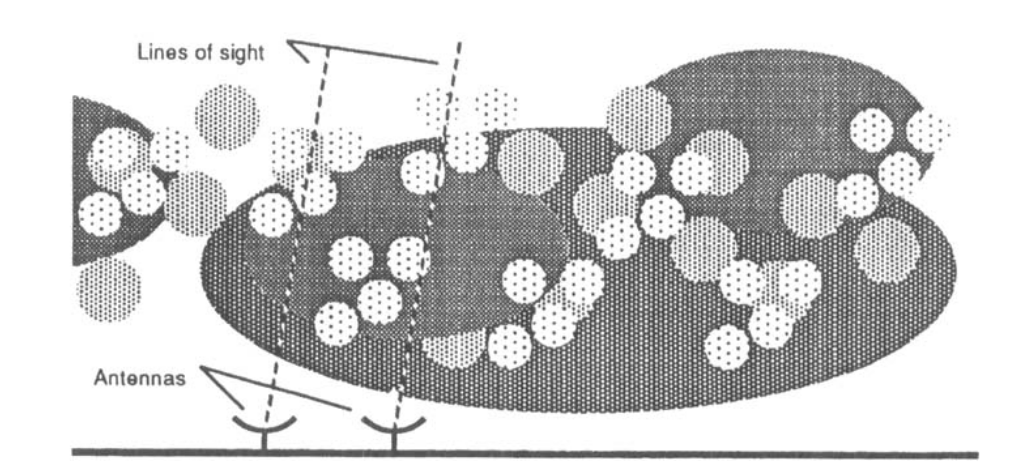
\includegraphics[height=60mm,width=120mm]{screen}
    \caption{A cartoon illustration of poorly mixed water vapour moving over a baseline (credit : Thompson et al, ibid) \label{phase:screen}}
\end{figure}

We can describe not only the differential fluctuations between two antennas but also the temporal fluctuations at a single antenna. Using the frozen screen assumption, that the timescale for distribution to evolve is much smaller than wind speed. The structure function becomes  $D(R)=D(t)|_{R=v \tau}$ where v is windspeed. In the case of VLBI, the distances between antennas are much larger than the correlation length of the turbulence, so in order to generate turbulence we generate a time series for each antenna. This is essentially a phase screen per antenna as the tropospheric corruption is constant across the field of view. A time series actually evades some  

Also assume a(l) constant until L.

One can write the variance of the phase $\sigma_\phi^2$ as a function of the structure function assuming that the observation is integrated over a time, T, (see Treuhaft and Lanyi (1986) appendix B for derivation)

\begin{equation}
\sigma^2_{\phi}(\tau) = (1/T)^2 \int_{0}^{T} (T-t) D_{\phi}(t) dt
\end{equation}

Writing the structure function, equation \ref{kolmogorov}, in terms of phase,
\begin{equation}
D_{\phi}(d)=a\left( \sec\theta \frac{2 \pi}{\lambda} d^{\beta} \right)^2  ,
\end{equation}
where a is a numerical constant depending on the site and the airmass is included. Performing the integration

\begin{equation}
\sigma_\phi (T)=\left[\frac{\sec\theta}{\beta^2 +3\beta +2}\right]( \frac{2 \pi}{\lambda}) a (v T)^{\beta}.
\end{equation}\\

Note that the power law index, $\beta$ falls off with increasing d and beyond a certain distance phases will become completely incoherent. Treuhaft and Lanyi (1986) show that in theory when $d<<L$, $\beta \approx 5/6$ and if $d>>L$,  $\beta \sim 1/3$ , varying continously and beyond a certain distance $\beta \to 0$.  \\
\\

\begin{figure}[h!]
\centering
    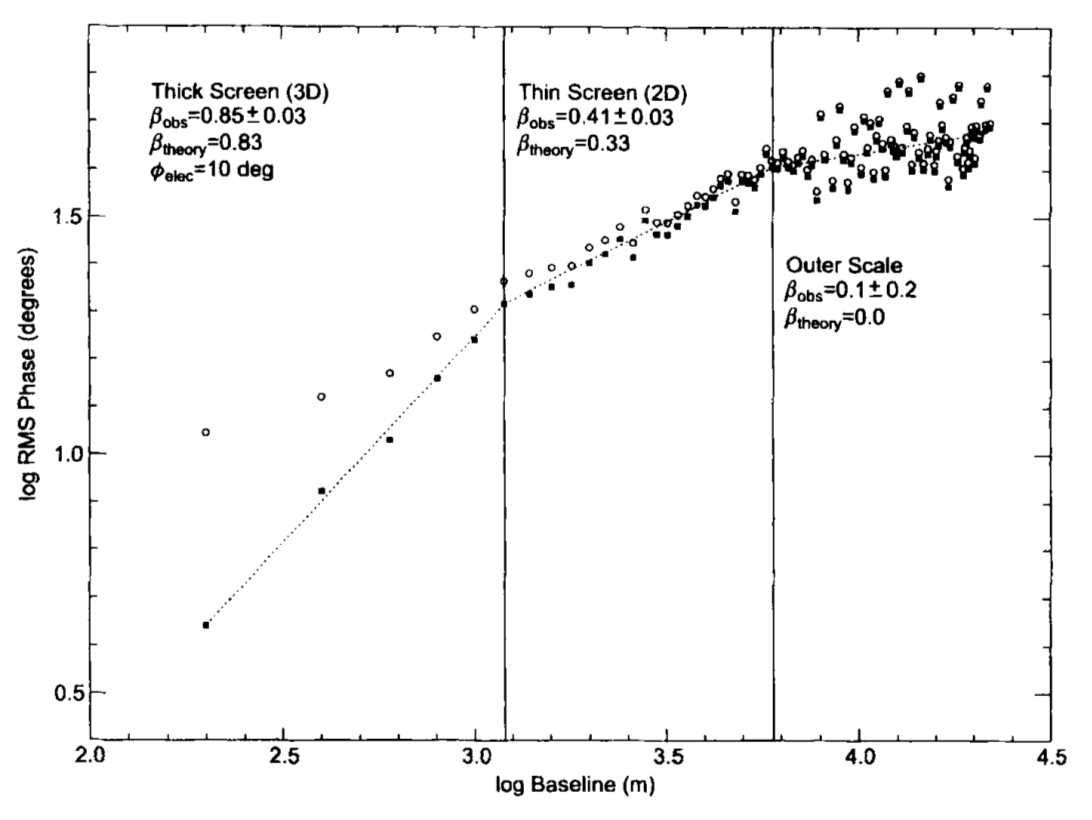
\includegraphics[scale=0.2]{screentransition}
    \caption{showing $\beta$ changes with distance on the phase screen. Note the three distinct regime but continous variation in between}
\end{figure}
In the regime of $d<<L$, $\beta \approx 2/3$

Often used to simulate phase screens is the spatial spectral power function (Thompson eq ) however because the field of view is so small, the phase screen shouldn't change therefore time seriesis better than simulating a phase screen because its resistant to coarseness sampling bias of the power spectrum which otherwise needs to be corrected for ( Lane et al, 1992)
\begin{figure}[h!]
\centering
    \includegraphics[height=60mm,width=120mm]{flow3}
    \caption{block diagram of the MeqSilhouette simulator }
\end{figure}

Treuft \& Lanyi (1987) $\beta$ varies with zenith angle and d.  at d<<h where h is the height of the troposphere $\sigma \sim (pathlength)^0.5$ but as d>>h $\sigma \sim pathlength$. Also need to address angle between wind and base.
 
allan variance useful for comparing tropospheric errors with other stochastic errors

for ALMA:
The timescale for changes in water vapour distribution is long compared to time for wind to carry features over array $v_w=10 m/s$

define $d_0$ where $\sigma = 1$~rad, i.e. phases are completely uncorrelated.

\begin{equation}
d_0 = 0.058 \lambda^\frac{6}{5}\sqrt{C_N^2 L}^\frac{-3}{5}
\end{equation}

\subsection{Instrumental}

\subsubsection{Thermal Noise}
%Pr 1 St 2
Review the TMS section on thermal noise basics.

Mild derivation of the thermal noise equation.
Does this properly take into account individual antenna noises that are correlated? Unexpectedly this implementation becomes important for the non-zero trop cp later.

\subsubsection{Antenna Pointing}
%Pr 1 St 2.  Take out implementation

All antennas suffer pointing errors to some degree due to a variety of factors including dish flexure due to gravity, wind and thermal loading, as well as drive mechanics. This corresponds to an offset primary beam, which should only translate to minor amplitude errors if the pointing error $\theta_{\rm PE}$ is significantly smaller than the primary beam (i.e. $\theta_{\rm PE} \ll \theta_{\rm PB}$). In the Measurement Equation formalism, this offset can be represented by a modified (shifted) primary beam pattern in the {\bf \it E}-Jones term 
\begin{equation}
{\bf E}_p(l,m) = {\bf E}(l_0 + \delta l_p, m_0 + \delta m_p),
\end{equation}
where $\delta l_p, \delta m_p$ correspond to the directional cosine offsets.


We investigate the effect of pointing errors on the 50~m (i.e. fully illuminated) LMT dish configured in an eight station VLBI array. The LMT has been measured to have an absolute pointing accuracy of $\sigma_{\rm abs} = 1-3$~arcsec, where smaller offsets occur when observing sources closer to zenith, and a tracking pointing accuracy $\sigma_{\rm track} < 1$~arcsec \footnote{http://www.lmtgtm.org/telescope/telescope-description/}. We explore the observational effect of these errors through three different pointing error models which explore different instructive and plausible scenarios. The LMT has been singled out as this may well serve as a reference station for the EHT array given its sensitivity and central geographic location. The source used is a circular Gaussian of characteristic size $\Theta_{\rm src}=50$ $\mu$-arcsec, located at the phase centre. For this investigation, as long as $\Theta_{\rm src} \ll \theta_{\rm PB}$, the exact structure of the source is unimportant. We approximate the LMT beam profile using an analytic WSRT beam model \citep{Popping_2008} with a factor of 2 increase in the beam factor $C$ to take into account the increased dish size
\begin{equation}
E(l, m) = \cos^3(C\nu \rho),\qquad   \rho = \sqrt{\delta l_p^2 + \delta m_p^2}
\end{equation}
where $C$ is a constant, with value $C \approx 130$~GHz$^{-1}$. Note that the power beam $EE^H$ becomes $\cos^6$, giving a $\rm{FWHM} = 6.5 $~arcsec. In Fig.~\ref{fig:pointing}, we show this for pointing accuracies spanning the range from $\rho \sim 0-4.5$~arcsec. 

In the first case we assume a constant pointing error and plot the RMS relative visibility amplitude error $\sigma_{\Delta V/V_0}$ on baselines to LMT, where $\Delta V = V_{\rm point} - V_{0}$, $V_{\rm point}$ and $V_{0}$ are the amplitude of the visibility with and without pointing errors respectively. This simulation is meant to be instructive as to the typical amplitude error in the simplest possible scenario.


Also interesting to consider is a slower, continuous time-variable pointing error associated with the tracking error $\sigma_{\rm track}$. Physically this could be attributed to changes in wind, thermal and gravitational loading which all change with telescope pointing direction and over the course of a typical few hour observation. Using the MeqTrees software package, such behaviour has been demonstrated to occur with the Westerbork Synthesis Radio Telescope (WSRT, \cite{Smirnov_2011c})\footnote{See also https://indico.skatelescope.org/event/\\171/session/9/contribution/20}. This is modeled as a sinusoid with period sampled from a uniform distribution between 0.5 and 6 hours, and a peak amplitude $A_{\rho} = \sqrt{2} \sigma_{\rho}$ , where the factor $\sqrt{2}$ relates the amplitude to the RMS for periodic zero mean waveforms. 


Whilst a stationary phase centre is tracked, the pointing error should evolve slowly and smoothly, however, in mm-VLBI observations the phase centre is often shifted to another source/calibrator. This would cause the pointing error to change abruptly, with an absolute pointing error $\sigma_{\rm abs}$. Source/calibrator change is scheduled every 5-10 minutes in a typical millimetre observation. The point is that even though EHT will be able to determine the pointing offset when observing a calibrator with well known structure, when the antennas slew back to a source (e.g. Sgr~A$^\star$) with less certain or variable source structure, the pointing error could change significantly. This is exacerbated by the scarcity of mm-wavelength calibrators, which are often widely separated from the source. We simulate this effect by re-sampling the pointing error every 10 minutes from a Gaussian of characteristic width equal to the quoted pointing error. We perform 50 realisations of the simulation for each pointing offset to generate reasonable uncertainties.




\subsubsection{Polarisation}
% Leave for now



